As data continues to increase in complexity and scale, data scientists are increasingly turning to machine learning to automatically make decisions.  However, when these decisions are applied to high-stakes domains such as medicine, law enforcement, and financial lending, it is critical for humans to understand the basis for these decisions.

% We analyze the effect of providing aggregation and navigation for instance level explanations on trust and the ability to generate diagnostic insights of predictive models.

Predictive modeling is an area of supervised machine learning which aims to predict outcomes from data.
Such models are trained on examples with a known ground truth.  In order to verify that a model generalizes well to unseen data, a hold-out data set with known ground truth is typically used to test the model after training.
This allows to detect problems with the model, such as over-fitting on the training data, \ie, the model learned a phenomenon that is only present in the training data, by measuring the gap in the accuracy between the training and the testing data.
However, sometimes a bias in the collected data affects both the training and the test data which makes it impossible to detect through accuracy alone.
A human understanding of the underlying data is needed.

For example, Caruana~\etal\cite{Caruana:2015:IMH:2783258.2788613} built an interpretable machine learning model to analyze mortality risk in patients diagnosed with Pneumonia.
After analyzing the model's behavior, Caruana~\etal detected that patients that additionally suffered from Asthma had a significantly lower mortality risk, according to the \emph{model} and supported by the data.
However, this finding goes against current medical knowledge, as the combination of Pneumonia and Asthma are associated with a significantly increased mortality risk.
In fact, the data was biased because these high-risk patients with Asthma were given special attention during their hospital visits which contributed to their lower mortality.  The presence of Asthma was not responsible for their improvement in health, but rather a systematic bias. 

\begin{figure}[t]
 \centering
 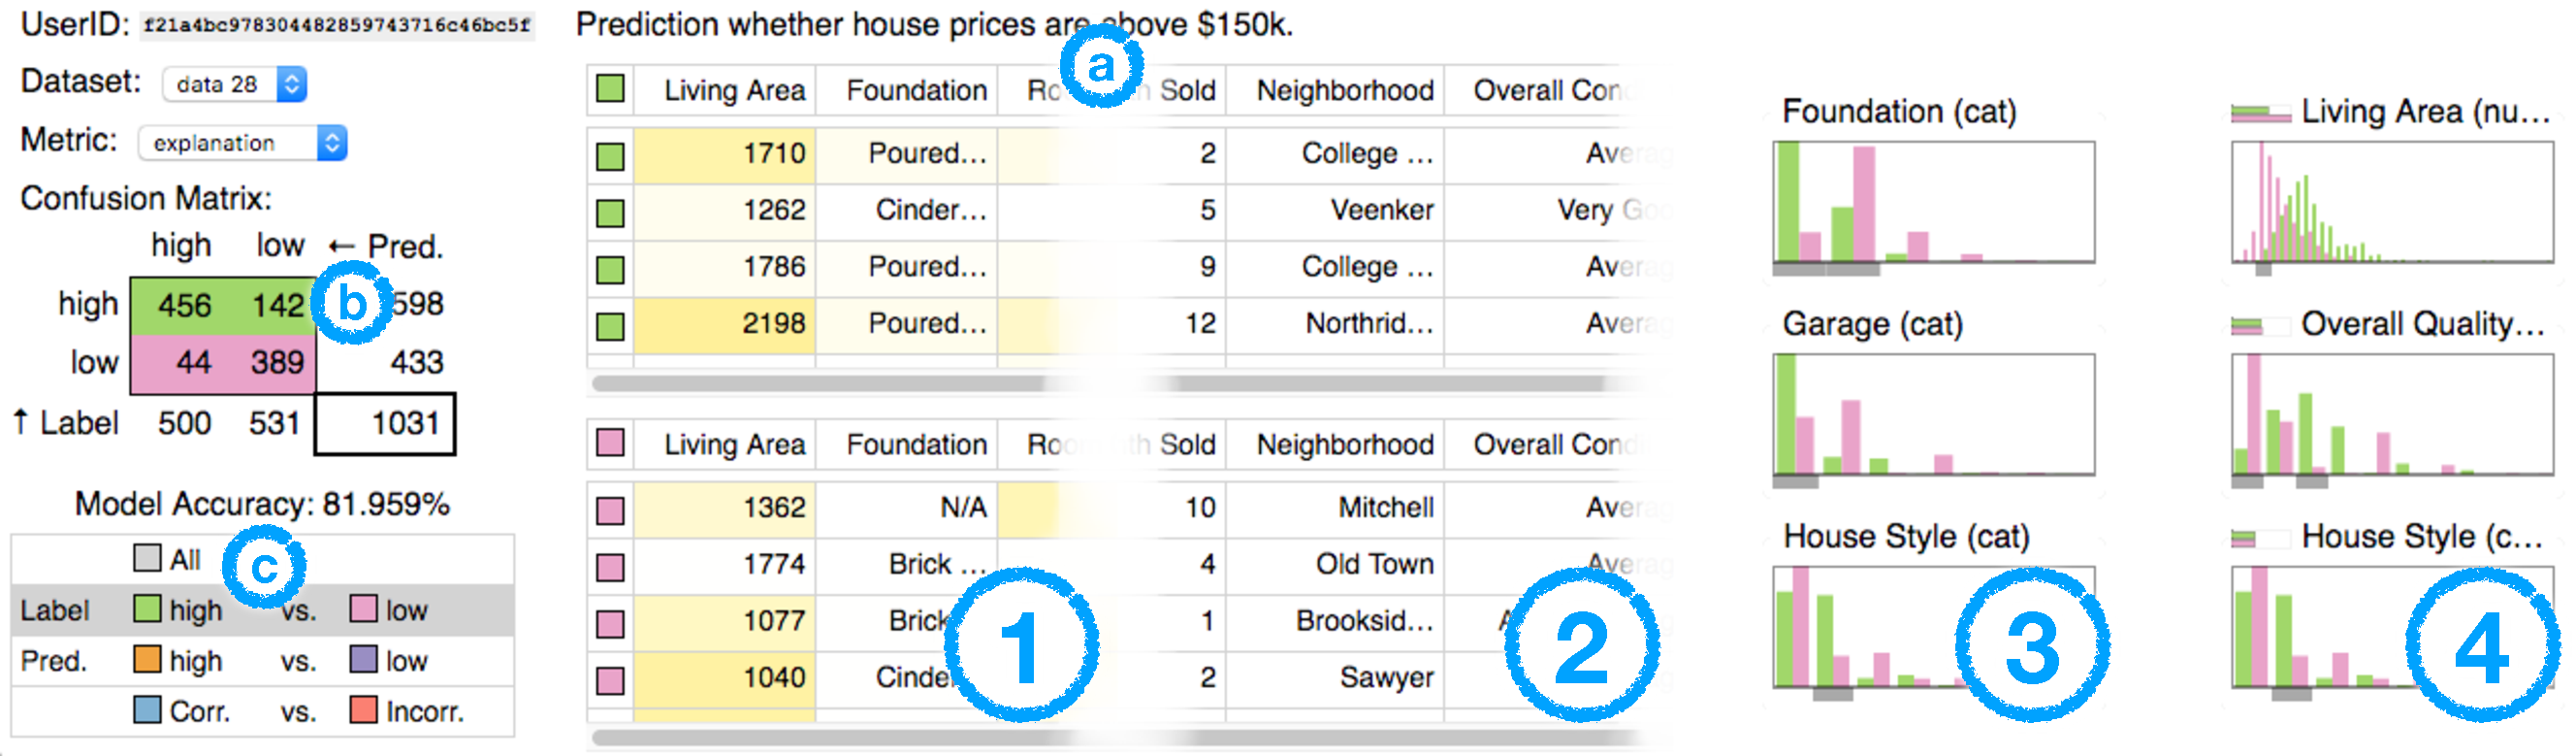
\includegraphics[width=\linewidth]{aggexplain/teaser.pdf}
 \caption[Showing the four study conditions.]{
Showing the four conditions of our study: (1) instance-level explanations; (2) only instances; (3) only aggregated features; (4) aggregated features with explanations.
On the left and the top are consistent parts of the user interface showing: (a) the problem description; (b) the confusion matrix; (c) the subset selector.
%\adam{This teaser is a bit confusing. Would it be better to just have the complete UI here and this figure later.}
% I keep it for now
 }
 \label{figs:teaser}
\end{figure}

Using the interpretable model and human expert knowledge, it was possible to detect this systematic bias in the data before deploying the model.
However, using interpretable machine learning algorithms typically penalizes their capacity, thus lowering the potential accuracy of the model \cite{Caruana:2015:IMH:2783258.2788613} or is only superficially more interpretable by being interpretable on a small scale but not for more complex tasks (\cite{2016arXiv160603490L,2016arXiv160605685K}).
As a way to interpret the behavior of machine learning models \emph{independently} from the used algorithm, black-box and more precisely, instance-level explanations recently became popular \cite{Martens:2014:EDD:2600518.2600523,DBLP:journals/corr/RibeiroSG16,krause2016interacting}.

However, such explanations are commonly reviewed by experts one-at-a-time.
This task becomes infeasible when dealing with thousands or more instances, also typical of real-world datasets.
To that extent, we propose a visual way of reviewing instance level explanations with the help of aggregation in combination with navigation.
This is implemented through the comparison of subsets of the test data under different conditions.

\begin{figure}[t]
\centering
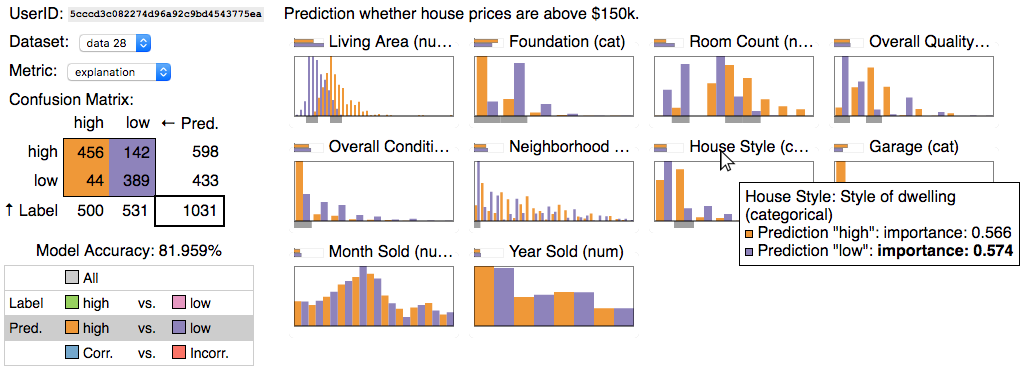
\includegraphics[width=\linewidth]{aggexplain/full_histogram}
\caption[The full interface illustrating the aggregated histogram view.]{
The full interface illustrating the aggregated histogram view.
The user is comparing the model's prediction of ``high'' house prices (orange) to the prediction of ``low'' prices (purple).
The user hovers over the feature ``House Style'' revealing a more detailed description, whether the feature is categorical or numeric, and the importance / feature weight for each of the subsets.
}
\label{figs:full_hist_view}
\end{figure}

We conducted a study comparing aggregated instance-level explanations to their individual counterparts.
Under both conditions different subsets of the test data could be compared by participants.
By providing models with both biased and unbiased data we were able to measure the trust of participants in the decisions made by the models and their ability to detect flaws in the underlying data for both methods.

Concretely, our contributions include a method for effectively comparing subset of a data set using histograms; using this method, a way to effectively aggregate instance-level explanations; and a study showing that this aggregation overcomes the potential harmfulness of instance-level explanations.
% \begin{itemize} %[leftmargin=*,noitemsep,nolistsep]
% \item \textbf{Design:} Techniques for Comparison,Y,Z. 
% \item \textbf{User Study:} Shows A,B,C
% \end{itemize}
% \todo{Fill in bulletpoints}

Following, we will first discuss related work in Section~\ref{sec:relatedwork} and then motivate the circumstances of our study further in Section~\ref{sec:motivation}.
We will propose our design for aggregating and comparing subsets of instance-level explanations in Section~\ref{sec:design}.
Afterwards we will describe the experimental setup in Section~\ref{sec:setup}.
The results of the study are provided in Section~\ref{sec:results} and their implications are discussed in Section~\ref{sec:ag_discussion}.
We then conclude in Section~\ref{sec:conclusion} and discuss future work.
